\chapter{Improvements to the Weather Research and Forecasting Model over First-Year Sea Ice}
\vspace{1 cm}
\begin{spacing}{1} \begin{quote} 
\noindent \emph{Current Arctic sea ice coverage levels (both annual and late summer) are at their lowest since at least 1850 (high confidence), and for late summer for the past 1000 years (medium confidence). Since the late 1970s, Arctic sea ice area and thickness have decreased in both summer and winter, with sea ice becoming younger, thinner and more dynamic (very high confidence).}\end{quote}
\hspace{6 cm} - IPCC Sixth Assessment Report, August 2021  
\end{spacing}
\vspace{1 cm}
\noindent 
\vspace{1 cm}\\

\section*{Abstract}

\begin{spacing}{1} \noindent Modeling sensible and latent heat flux over first-year sea ice is becoming more important as young sea ice begins to dominate the polar regions. In-situ atmospheric observations over sea ice are rare, as field experiments can be dangerous and expensive, resulting in a lack of validation and tuning data for modeling in these regions. The Norwegian Young Sea Ice Experiment (N-ICE) observed atmospheric conditions from January to June 2015, providing valuable observational data. Eddy covariance measurements from N-ICE were processed through the LI-COR’s EddyPro 7 software to estimate surface heat fluxes over the first-year ice using the eddy covariance method. The Noah Land Surface Model (LSM) used to calculate surface fluxes in Weather Research and Forecasting (WRF) model currently uses the bulk approach over sea ice, which requires estimations of the Monin-Obukhov scaling and stability parameters. These parameters are dependent on wind, potential temperature gradients, and surface stability. The cold surface often results in a strongly stable surface layer, a characteristic unique to the polar regions, presenting potential errors in the stability regimes used to estimate these parameters. Results from the Polar WRF over the N-ICE domain disagree with those directly calculated from the measurements. The magnitude of these differences reached greater than 40 $Wm^{-2}$ at times. In this study, sensible and latent heat flux from N-ICE calculated using the eddy covariance method (EddyPro) is compared to those calculated using the bulk method (both calculated offline and from the Noah LSM in WRF). A sensitivity study is also presented examining the often empirically derived scaling and stability parameters used in the bulk method calculations, with recommendations for these values over first-year sea ice.
\end{spacing}

\doublespacing
\section{Introduction}

The global climate is heavily influenced by processes that occur in the Arctic. A lack of observation has led to difficulty in understanding atmospheric processes in polar regions \citep{persson:2002}. The IPCC \citep{IPCC:14} lists high to very high confidence in observed changes in marine and terrestrial ecosystems, food production, and health/economics in the polar regions due to climate change. Both the Arctic and Antarctic are projected to continue warming more quickly than the global mean temperature. There is high confidence that year-round sea ice extent has been decreasing since before 1970 and will continue to decrease in the future. The IPCC \citep{IPCC:14} indicates that a changing climate may have large impacts on indigenous people, marine mammals, and coastal ecosystems in the Arctic. However, there are many observational uncertainties, such as in anthropogenic forcings in the polar regions, leading to low confidence \citep{IPCC:14}. Observational uncertainties in these regions stem from the harsh conditions and difficulty in deploying ground-based instruments.

Changes occurring in the Arctic modify the atmospheric circulation, impacting both cloudiness and radiation at the surface \citep{zhang:2008}. According to \citet{stroeve:2007}, many CMIP5 members show that there may be ice-free conditions within the next couple of years. In addition, Maslanik et al. \citep{maslanik:2007} states that the ice cover can be very sensitive to temperature changes, resulting in large and rapid changes in sea ice extent. Temperatures in the Arctic have increased much more quickly than those elsewhere on the planet, averaging 2 to 3 times faster than the global average, with longer melt seasons and more variability in snow cover \citep{sledd:2019, AACI:05}. In addition, multi-year ice is disappearing, and being replaced with thin, single-year ice. This movement toward a new ice regime has been referred to as a shift toward a new climate state in the Arctic \citep{verlinde:2007}.  

Arctic amplification is a significant factor in the poles warming more quickly than other parts of the globe. Arctic amplification modifies the surface energy budget. The amplification occurs because as the Arctic warms, the albedo decreases. The ice-albedo feedback occurs as warmer temperatures cause an increase in ice melt. The albedo of the open ocean or bare land is much lower than that of sea ice or snow, resulting in greater absorption of incoming solar radiation. As the open ocean (or bare surface) absorbs more shortwave radiation, the ocean (land) surface heats, resulting in a greater extent of melt, and therefore further amplification of the ice-albedo feedback. Clouds are an important factor to consider when observing this feedback, as they can enhance or slow surface melt by modifying the energy balance. The presence of clouds can reduce the impacts of sea ice loss by reflecting shortwave radiation away from the earth due to their high albedo, therefore reducing the amount of radiation absorbed by the low albedo surface. \citet{hwang:2018} states that clouds can reduce the ice-albedo feedback at the surface by around 0.44 $Wm^{-2}$, as was seen in 2007 when a record low sea ice extent was observed \citep{hwang:2018, sledd:2019}.

Cloud radiation feedback is more dynamic than ice-albedo feedback in the sense that it can be either positive or negative depending on a variety of influences. Clouds change the surface temperature by modifying both the shortwave and longwave radiation reaching the surface. Cloud microphysics, such as phase and particle size, as well as macrophysics, including fractional coverage, cloud height, and thickness, can influence the amount of radiation reaching the surface and, in turn, influence the impact of the cloud-radiation feedback \citep{uttal:2002}. This relationship is nonlinear and depends on both cloud and sea ice characteristics \citep{intrieri:2002}.

Clouds, as stated above, can modify both the radiation budget and impact the ice-albedo feedback. The influence of clouds is magnified by the high surface albedo and the lack of atmospheric moisture \citep{shupe:2003}. Clouds have the greatest potential to modify heat exchange in the Arctic \citep{intrieri:2002}. While we do have some estimates on how much the clouds can impact these feedbacks, more information is needed to quantify the exact influence. \citet{sledd:2019} states that the clouds are the most important driver in changes in top-of-atmosphere albedo over the entire globe, including at the poles, regardless of the high surface albedo. Cloud characteristics were shown to directly impact the ice thickness in studies by \citet{curry:1992, beesley:2007}.  

The impact of clouds is often quantified using cloud radiative forcing (CRF). The CRF describes how clouds modify the radiation at the surface by taking the difference between the observed radiation and the clear-sky radiation \citep{ramanathan:1989}. When positive radiative forcing is observed, there is a surplus of net radiation at the surface, and warming occurs. When the CRF is negative, cooling occurs at the surface. During clear skies, CRF should equal zero, as the actual radiation should be the same as the estimation of clear-sky radiation. Clear-sky radiation is often calculated from a radiative transfer model or estimated using observed clear-sky times.

Net cloud radiative forcing is a balance of surface warming and cooling due to modifications in radiation as a result of cloud cover. \citet{curry:1992, intrieri:2002} found that in the Arctic, clouds warm the surface over the entire year (have a positive cloud radiative forcing) except for in mid-July when the sun is highest above the horizon. This nearly year-round warming is due to the small amount of shortwave radiation. When there is solar radiation present, the low sun elevation angle and high surface albedo reflect much of the shortwave radiation away. In addition, the low-level clouds are often emitting longwave radiation at warmer temperatures than the ice surface due to surface temperature inversions \citep{shupe:2003}.

Models in the polar regions have the largest uncertainties relative to other parts of the Earth \citep{holland:2003, AACI:05}. Models have difficulty simulating radiation accurately during times of thick clouds. A likely reason for this is the model’s inability to estimate the number of liquid phase drops within the cloud \citep{graham:2017}. A surface inversion often persists over the winter months and processes under these stable conditions are not well understood or modeled \citep{tastula:2012}. In the summer, these inversions are often elevated compared to the wintertime surface inversions \citep{serreze:1992}. Models, however, are integral in understanding the processes occurring in the poles, particularly the radiation.  Unfortunately, few field experiments collecting data for validation exist.

Reanalysis products are often used to study the Arctic climate. This poses a challenge as they are not as thoroughly verified as in other locations due to the extreme climate and dark winters preventing accurate, long-term, multi-season, in-situ, and satellite measurements. Biases in clouds result in difficulties in resolving the surface energy budget. Recent studies have shown that when compared with surface observations, reanalysis have large biases in cloud properties (liquid/ice water path, fraction). A number of field experiments have shown that mixed-phase clouds are dominant in autumn through spring in the lower levels at high latitudes \citep{intrieri:2002, wang:2005}. Cloud micro- and macrophysics are closely tied to the surface energy budget, but parameterizations of such are not well developed in models. Particularly in the Arctic, the radiative properties of clouds and how they are parameterized in models are of importance to modeling the surface energy budget. 

The  Norwegian Young Sea Ice Experiment (N-ICE, described in section 3) field campaign was the first winter field experiment in the Arctic since the Surface Heat Budget of the Arctic (SHEBA) experiment, taking place onboard a research vessel frozen into Arctic sea ice. SHEBA’s primary goals were to observe the surface energy budget, ice mass balance, and ocean-ice-atmosphere interactions in the Arctic during a year-long period from October 1997 to October 1998. Much like N-ICE, SHEBA was motivated by changes in the Arctic and the need for a better understanding of physical processes in the polar regions \citep{randall:1998}. A secondary objective of SHEBA was to improve model simulations of the Arctic for use in global climate models \citep{uttal:2002}. Both the ice-albedo feedback and the cloud-radiation feedback were extensively studied using datasets collected during this field experiment. However, this experiment occurred 18 years prior to N-ICE and in a different location of the Arctic, influenced by different synoptic conditions. 

\section{Methods}

The idealized version of the Weather Research and Forecasting model was used to test the sensitivity of the model to changes in the set parameters found in LANDUSE.TBL. Idealized model simulations are used to create an "idealized" atmosphere at a point in space. These runs are not as computationally expensive or as time-consuming as using the full model, so they are often utilized for sensitivity studies.

The LANDUSE.TBL file is one of three tables used in WRF to set constants. This file table specifies constants dealing with the surface-atmosphere interface within the mode, including the surface albedo, surface moisture availability, surface emissivity, surface roughness, thermal inertia constant, snow cover effect, and surface heat capacity. There are different "sections" within this table. Much like choosing different physical schemes based on expected conditions, these sections each have different sets of values determined from varying experiments, and many sections specify values for summer and winter separately. 

\begin{table}[h]
\footnotesize
\center
\centering
\doublespacing
\begin{tabular}{| c | c | c | c | c |  c |}
\hline
 \rowcolor[HTML]{ECECEC} \rule{0pt}{35pt} \multirow{-3}{*}{\textbf{Section}} & \multirow{-3}{*}{\textbf{Season}} & \multirow{-3}{*}{\textbf{\shortstack{Albedo\\ $(\%)$}}} & \multirow{-3}{*}{\textbf{\shortstack{Surface \\ Emissivity\\ $(\%)$}}} & \multirow{-3}{*}{\textbf{\shortstack{Surface \\ Roughness}}} & \multirow{-3}{*}{\textbf{Category}} \\ \hline
\rule{0pt}{12pt} & Summer & 55 & .95 & 5 &  \\
\rule{0pt}{12pt} \multirow{-2.5}{*}{\textbf{OLD}} & Winter & 70 & .95 & 5 & \multirow{-2.5}{*}{\shortstack{Permanent \\ Ice}} \\ \hline
\rule{0pt}{12pt} & Summer & 55 & .95 & .1 &  \\
\rule{0pt}{12pt} \multirow{-2.5}{*}{\textbf{USGS}} & Winter & 70 & .95 & .1 & \multirow{-2.5}{*}{\shortstack{Snow or Ice}} \\ \hline
\rule{0pt}{12pt} & Summer & 55 & .95 & .1 &  \\
\rule{0pt}{12pt} \multirow{-2.5}{*}{\textbf{\shortstack{MODIFIED IGBP \\ MODIS NOAH}}} & Winter & 70 & .95 & .1 & \multirow{-2.5}{*}{\shortstack{Snow or Ice}} \\ \hline
\rule{0pt}{12pt} & Summer & 55 & .95 & 5 &  \\
\rule{0pt}{12pt}\multirow{-2.5}{*}{\textbf{SiB}} & Winter & 70 & .95 & 5 & \multirow{-2.5}{*}{\shortstack{Ice Cap \\ and Glacier}} \\ \hline
\rule{0pt}{12pt} & Summer & 55 & .95 & 1 &   \\
\rule{0pt}{12pt}\multirow{-2.5}{*}{\textbf{MODIS}} & Winter & 55 & .98 & 1 & \multirow{-2.5}{*}{\shortstack{Snow and Ice}}  \\ \hline
\rule{0pt}{12pt} & Summer & 55 & .95 & .1 &   \\
\rule{0pt}{12pt}\multirow{-2.5}{*}{\textbf{SSIB}} & Winter & 70 & .95 & .1 & \multirow{-2.5}{*}{\shortstack{Snow or Ice}}  \\ \hline
 \rule{0pt}{12pt} & Summer & 60 & .95 & 1.2 & \\
\rule{0pt}{12pt} \multirow{-2.5}{*}{\textbf{NLCD40}} & Winter & 60 & .95 & 1.2 & \multirow{-2.5}{*}{\shortstack{Permanent \\ Snow and Ice}} \\ \hline
\rule{0pt}{15pt} \textbf{LW12} & All & 70 & .95 & 5 & \shortstack{Snow and Ice} \\ \hline
\end{tabular}
\caption{Current settings for snow and ice in the LANDUSE.TBL file used by WRF.}
\label{tab:wrf:landusetbl}
\end{table}

Table \ref{tab:wrf:landusetbl} shows all sections in the LANDUSE.TBL file for any sort of snow or ice surface. This table does not include the surface moisture availability, the thermal inertia constant, or the snow cover effect, as these were held constant at 95$\%$, 5, and 0, respectively. These have not been included in this table as they are not the focus of this study and were kept constant. The section of this table the model reads is specified within the model setup file. Previous modeling studies (chapter 2) used the USGS section of this table, so this study also uses this section.

\subsection{Changing Constants in LANDUSE.TBL}

\subsubsection{Roughness}

Roughness length ($z_{0}$) is defined in Eq. \ref{eq:z0} and requires wind speed ($U_{1}$ and $U_{2}$) at two heights ($z_{1}$ and $z_{2}$), the von K\'{a}rm\'{a}n constant (0.4), and the friction velocity. Wind speed was measured at three heights during N-ICE. For this application, we will be using the 2 $m$ measurement as $U_{1}$ and the 10 $m$ measurement has $U_{2}$. Calculations were also done using 2 $m$ and 4 $m$ with similar results, so 10 $m$ was used for $z_{2}$. The friction velocity ($u*$) is closely related to the roughness length and is discussed in depth later. For this part of the study, the friction velocity value from the EddyPro flux data was used. 

\begin{equation}\label{eq:z0}
 z_{0} = \frac{(z_{2}-z_{1})}{[exp(\frac{kU_{2}}{u*}) - exp(\frac{kU_{1}}{u*})]} 
\end{equation}

The mean roughness length for N-ICE is 0.00124 $m$ when calculated using Eq. \ref{eq:z0}. EddyPro defines the roughness length as 0.15 times the canopy height. Since our canopy height has been entered into the program as 0, EddyPro also calculates our roughness length values to be 0.001 for the entire experiment. The section in Table \ref{tab:wrf:landusetbl} being used already has the lowest friction velocity of all sections, but it is still higher than that calculated from observations taken at N-ICE. 

\subsubsection{Albedo}

Albedo was calculated at N-ICE by taking the ratio of upward to downward shortwave radiation. More about the albedo measurements can be found in \citet{walden:2017}. A breakdown of the albedo measurements for each floe is seen in Table \ref{tab:albedos}. No albedo is listed for the first Floe as there was no shortwave radiation during this period. 

\begin{table}[h]
\centering
\footnotesize
\doublespacing 
{
\begin{tabular}{| c | c |}
 \hline
\rowcolor[HTML]{F3F3F3} \textbf{Floe} & \textbf{Albedo ($\%$)} \\
\hline
2 & 86 \\
3 & 82 \\
4 & 78 \\
 \hline
\end{tabular}}
\caption{Average albedo measured at N-ICE. Floe 1 is not included as albedo was calculated using shortwave radiation measurements, and the sun had not yet risen on Floe 1.}
\label{tab:albedos}
\end{table}

Albedo values specified in Table \ref{tab:wrf:landusetbl} do not exceed 70 $\%$, but even the lowest albedos measured at N-ICE were above 70 $\%$. Increasing the albedo would increase the amount of shortwave radiation being reflected away from the surface, changing the shortwave energy balance. In addition, less energy is being absorbed into the surface than is occurring in the model. This could result in errors elsewhere (for example, in the latent heat flux) as the energy budget in the model attempts to balance itself. The albedo values in Floe 2 can be taken to represent the winter albedo, and an average of all values in Floes 3 and 4 (81 $\%$) was used for the summer albedo.

\subsubsection{Surface Heat Capacity}

The surface heat capacity of sea ice is shown in Eq. \ref{ch5:c}. In this equation, $c$ is the heat capacity in $\frac{J}{kg K}$. It requires the salinity of the ice ($S$, $ppt$), the sea ice temperature ($T$, $K$), the heat capacity of fresh ice ($c_{0}$, $2054 J(kg K)^{-1}$), the latent heat of fusion ($L_{i}$, $3.340 \times 10^{5} Jkg^{-1}$), and the ocean freezing temperature constant ($\mu$, 0.054 $^{\circ}C~ppt^{-1}$, selected considering salinity). 

\begin{equation}\label{ch5:c}
c = c_{0} + \frac{L_{i}\mu S}{T^{2}}
\end{equation}

Ice cores were taken at N-ICE to measure ice temperature and salinity. Mean sea ice surface temperatures for winter and spring were -22.77 $^{\circ}C$ and -4.09 $^{\circ}C$, respectively. In the winter, ice surface temperature had a large range and varied as much as 30 $^{\circ}C$ in the course of one month. In the spring, surface temperatures were much more consistent, and showed a slow increase to freezing.

Salinity varied from 2 $g~kg^{-1}$ to 11 $g~kg^{-1}$ during both winter and spring, with little difference in the season averages. The mean salinity was 6.08 $g~kg^{-1}$ for the entire experiment. Using Eq. \ref{ch5:c} with these values gives surface heat capacity values of approximately $1.83 \times 10^{6}$. This is several orders of magnitude larger than what is specified in LANDUSE.TBL.

\subsection{Flux Equations}

In Chapter 5, we discuss two ways to calculate the sensible and latent heat flux over first-year sea ice: using a bulk flux algorithm \citep{foken:2008} and using the Maximum Entropy Potential (MEP) method \citep{zhang:2021, wang:2014, wang:2009} Both methods require some assumptions and scaling parameters that are generally formulated empirically and based on the atmospheric stability at the surface. 

In the WRF model, the heat and moisture fluxes are calculated in the surface layer (SL) scheme and land surface model (LSM). These schemes also calculate the upward longwave and shortwave radiation \citep{dudhia:2014, skamarock:2019} The downward components of shortwave and longwave radiation are calculated in the radiation scheme. In this study, we focus on the components that were formulated in the SL scheme and land surface model. 

The Polar WRF sensitivity study in Chapter 3 used the Revised MM5 scheme \citep{paulson:1970, dyer:1970, webb:1970, beljaars:1994} and ETA Similarity scheme for the SL scheme depending on the boundary layer (PBL) scheme selection. The ETA Similarity SL scheme was only used with the Mellor–Yamada–Janji PBL scheme, as this is required by the model. In this study, we take a deeper look into the Revised MM5 SL scheme. In general, SL schemes calculate the surface exchange coefficients (Eq. \ref{eq:wrf:psi}, using Eq. \ref{eq:wrf:zal} and Eq. \ref{eq:wrf:rb}), roughness lengths, and friction velocity \citep{dudhia:2014}. Monin-Obukhov similarity theory is used in every SL scheme currently available in the model. 

\begin{equation}\label{eq:wrf:psi}
\varphi_{m} = 
\varphi_{h} = \begin{cases} 
0 & \text{    } R_{b} > 0.2 \\ 
-5 \frac{z_{a}}{L} & \text{    } 0.2 > R_{b} > 0 \\ 
0 & \text{    } R_{b} < 0 \\ 
\end{cases}
\end{equation}

The scaling parameters defined in \ref{eq:wrf:psi} depend on the near-surface stability. The model uses the bulk Richardson number ($R_{b}$, Eq. \ref{eq:wrf:rb}) to define three stability regimes for which different relationships apply. These equations use the Richardson number ($R_{i}$, Eq. \ref{eq:wrf:ri}, Obukhov length ($L$), vertical wind sheer ($S_{i}$), wind speed at 2 $m$ above the ground ($V_{a}$), the roughness length ($z_{0$), and potential temperature ($\theta_{g}$, $\theta_{a}$, $\theta_{i+0.5}$ and $\theta_{i-0.5}$) at the ground level, the first level, halfway between ground and first level, and halfway between the first level and second level ($z_{g}$, $z_{a}$, $z_{i+0.5}$ and $z_{i-0.5}$). 

\begin{equation}\label{eq:wrf:zal}
\frac{z_{a}}{L} = \begin{cases} 
0 & \text{    } R_{b} > 0.2 \\ 
\frac{R_{b}}{1-5R_{b}}ln(\frac{z_{a}}{z_{0}}) & \text{    } 0.2 > R_{b} > 0 \\ 
R_{i} ( z_{1} ) & \text{    }R_{b} < 0  \\ 
\end{cases}
\end{equation}

\begin{equation}\label{eq:wrf:rb}
R_{b} = \frac{gz_{a}}{\theta_{a}}\frac{\theta_{a} - \theta_{g}}{(V_{a})^{2}}
\end{equation}

\begin{equation}\label{eq:wrf:ri}
R_{i} = \frac{g}{\theta_{a}S_{i}^{2}} \frac{\theta_{i+.5} - \theta_{i-.5}}{z_{i+.5} - z_{i-.5}}
\end{equation}


The Noah LSM \citep{chen:2001} was used in all model runs in Chapter 3 and is the LSM used for this study. Polar WRF modifies the Noah LSM for optimized use over the Arctic, including improvements to the surface energy balance and sea ice \citep{hines:2015, bromwich:2009}. The LSM uses atmospheric information from the SL scheme and precipitation/radiation from the cloud microphysics (CM) and convective schemes to calculate the vertical transport, fluxes (sensible and latent shown in Eq. \ref{eq:wrf:h}, \ref{eq:wrf:e}) in the lowest layers of the atmosphere. Friction velocity (Eq. \ref{eq:wrf:ustar}) and roughness length (Eq. \ref{eq:wrf:z0}). The Noah LSM does this using 4 soil temperature and moisture layers \citep{dudhia:2014, skamarock:2019} This particular LSM also can predict soil ice and fractional snow cover \cite{chen:2001}. 

\begin{equation}\label{eq:wrf:h}
H = \rho c_{p} u_{*} \theta_{*} = \rho c_{p} C_{hs} \delta \theta
\end{equation}

\begin{equation}\label{eq:wrf:chs}
C_{hs} = \frac{\kappa u_{*}}{ln (\frac{z}{z_{0}}) - \varphi_{h}}
\end{equation}

\begin{equation}\label{eq:wrf:ustar}
u_{*} = \frac{\kappa V_{r}}{ln(\frac{z_{r}}{z_{0}}) - \varphi_{m}}
\end{equation}

\begin{equation}\label{eq:wrf:thetastar}
\theta_{*} = \frac{\kappa \delta \theta}{ln(\frac{z_{r}}{z_{0h}}) - \varphi_{h}} 
\end{equation}

\begin{equation}\label{eq:wrf:e}
E = \rho u_{*} q_{*}
\end{equation}

\begin{equation}\label{eq:wrf:q*}
q_{*} = \frac{k \delta q}{ln(\frac{z_{r}}{z_{0q}}) - \varphi_{h}}
\end{equation}

To calculate the sensible heat flux, the model must also calculate the surface scaling parameter ($\varphi$), and the transfer equation ($C_{hs}$, Eq. \ref{eq:wrf:chs}). Additionally, values must be specified for the air density ($\rho$), and the heat capacity at constant pressure for dry air ($c_{p}$), and the temperature roughness length ($z_{0h}$). Knowledge of the moisture roughness length ($z_{0q}$) is required for the latent heat flux and is calculated within the model code. Note that the flux equations use $r$ as a subscript indicating the reference height, while the stability equations use layers.

\subsubsection{Friction Velocity and Roughness Length}

Before we can calculate the friction velocity, we must calculate the roughness length. The function within the LSM requires the snow cover, background roughness length, snow height, the fraction of snow under the canopy, ground snow cover, annual max vegetation fraction, and an option to improve the vegetation-snow interface. Our location has no vegetation, so we can ignore those variables, leaving us with only the background roughness length ($Z_{0brd}$), snow height ($SN_{H}$), and snow cover fraction ($SN_{COVR}$) to estimate. This equation is shown in Eq. \ref{eq:wrf:rl}.

\begin{equation}\label{eq:wrf:rl}
Z_{0} = (1 - SN_{COVR}) Z_{0brd} + SN_{COVR}) \space Z_{0eff}
\end{equation}

$Z0_{eff}$ is the effective roughness length and depends on the snow cover. If the snow height is greater than seven times the background roughness length, the effective roughness length is 0.001 $m$. Otherwise, the effective roughness length is estimated using the following equation:

\begin{equation}\label{eq:wrf:rleff}
Z0_{eff} = \frac{7Z_{0brd}-SN_{H}}{7}
\end{equation}

The next thing to estimate is the background roughness length ($Z_{0brd}$). \citet{untersteiner:1965} estimated the average roughness length of sea ice to be about 0.02 $cm$. This is the value used below and means that for every snow depth deeper than 0.0014 $m$ (or 0.14 $cm$), $Z_{0eff} = 0.001$. Next, we must make a decision about the snow cover fraction. Our location is fairly small, and we know all measurements were taken over sea ice, so we assume 100$\%$ snow cover fraction for the entire experiment. Using these estimations with Eq. \ref{eq:wrf:rl} and \ref{eq:wrf:rleff}, we get an average roughness length of 0.001 $m$ for the entire observation period. 


The surface exchange coefficients for heat and moisture are also required for roughness length and are defined in the SL scheme. The equations used here depend on the difference between the potential temperature at the surface and the first level above the ground. If this difference is greater than 0.00005, Eq. \ref{eq:flhx} is used to calculate the heat exchange coefficient, otherwise, the value is zero. The moisture exchange coefficient is defined by Eq. \ref{eq:flqc}. 

\begin{equation}\label{eq:flhx}
F_{LHX} = \frac{c_{p} * \rho u^{*} T^{*}}{(\theta_{z} - \theta_{g})}
\end{equation}

\begin{equation}\label{eq:flqc}
F_{LQC} = \frac{\rho M_{avail} u^{*} \kappa}{D_{Q}}
\end{equation}

$M_{avail}$ in Eq. \ref{eq:flqc} is the surface moisture availability (between zero and 1). For our case, we will assume this value is 1. $D_{Q}$ is a value defined with the friction velocity in the SL scheme. This depends on the stability and friction velocity. They are already calculated within the same function as the sensible and latent heat flux. Changes in Eq. \ref{eq:flqc} do not influence friction velocity. Eq. \ref{eq:flhx}, however, does.

\section{Results}

\subsection{LANDUSE.TBL Changes}

\begin{table}[h]
\centering
\footnotesize
{
\begin{tabular}{| c | c | c | c | c | c | c |}
\hline
\rowcolor[HTML]{F3F3F3} & \multicolumn{2}{c |}{\textbf{Winter Cloudy}} & \multicolumn{2}{ c | }{\textbf{Spring Cloudy}} & \multicolumn{2}{ c |}{\textbf{Spring Clear}} \\
\rowcolor[HTML]{F3F3F3} & \textbf{Modified} & \textbf{Original} & \textbf{Modified} & \textbf{Original} & \textbf{Modified} & \textbf{Original} \\
\hline
\textbf{Latent} & 12.13 & 13.52 & 1.60 & -0.20 & 3.98 & 4.81 \\
\textbf{Sensible} & 38.11 & 47.10 & -3.86 & -9.81 & -2.25 & 0.23 \\
\textbf{Downward Longwave} & -0.19 & 2.48 & -54.83 & 0.34 & -36.17 & -8.15 \\
\textbf{Upwawrd Longwave} & 6.50 & -1.23 & -11.69 & -19.14 & -5.58 & -13.31 \\
\textbf{Downward Shortwave} & & & 111.15 & 50.20 & 50.40 & 13.39 \\
\textbf{Upward Shortwave} & & & 81.96 & 33.21 & 48.41 & 15.04 \\
\hline
\end{tabular}}
\caption{Mean model biases ($Wm^{-2}$) for each idealized case study with both the modified (left) and original (right) runs.}
\label{tab:wrf:meanbias}
\end{table}

The model was run twice, once with the default LANDUSE.TBL options (Table \ref{tab:wrf:landusetbl}, USGS section) and once with values calculated for N-ICE. Table \ref{tab:wrf:recommendations} shows the values calculated above that were used in the modified LANDUSE.TBL. Everything else was held constant and ECMWF was used as the input dataset. The WRF model code is written in FORTRAN and has different files for each scheme. The SF scheme FORTRAN code has been translated to a stand-alone Python code allowing us to easily modify and run the code. 

\begin{table}[h]
\centering
\footnotesize
\doublespacing
{
\begin{tabular}{| c | c | c | c | c | c | c |}
 \hline
     \rowcolor[HTML]{F3F3F3} \rule{0pt}{35pt}  
     \multirow{-2}{*}{\textbf{Section}}  
     & \multirow{-2}{*}{\textbf{Season}}  
     & \multirow{-2}{*}{\shortstack{\textbf{Albedo} \\  $(\%)$}}  
     & \multirow{-2}{*}{\shortstack{\textbf{Surface} \\ \textbf{Emissivity} \\ $(\%)$}}  
     & \multirow{-2}{*}{\shortstack{\textbf{Surface} \\
     \textbf{Roughness}}} 
     & \multirow{-2}{*}{\shortstack{\textbf{Thermal} \\ \textbf{Inertia} \\ \textbf{Constant}}}  & \multirow{-2}{*}{\shortstack{\textbf{Surface Heat} \\ \textbf{Capacity} \\ $(J~m^{-3} K^{-1})$}}  \\
 \hline
\textbf{NICE}  & Winter  & 86 & .98 & .001 & 5 & $1.8 \times 10^{6}$ \\
 \textbf{NICE}     & Summer  & 81 & .98 & .001 & 5 & $1.8 \times 10^{6}$ \\
  \hline
\end{tabular}}
\caption{Recommended changes to the LANDUSE.TBL file for simulations over first-year sea ice. Original LANDUSE.TBL file settings for snow/ice can be seen in Table \ref{tab:wrf:landusetbl}}
\label{tab:wrf:recommendations}
\end{table}

\begin{figure}[h]
    \centering
    \doublespacing
    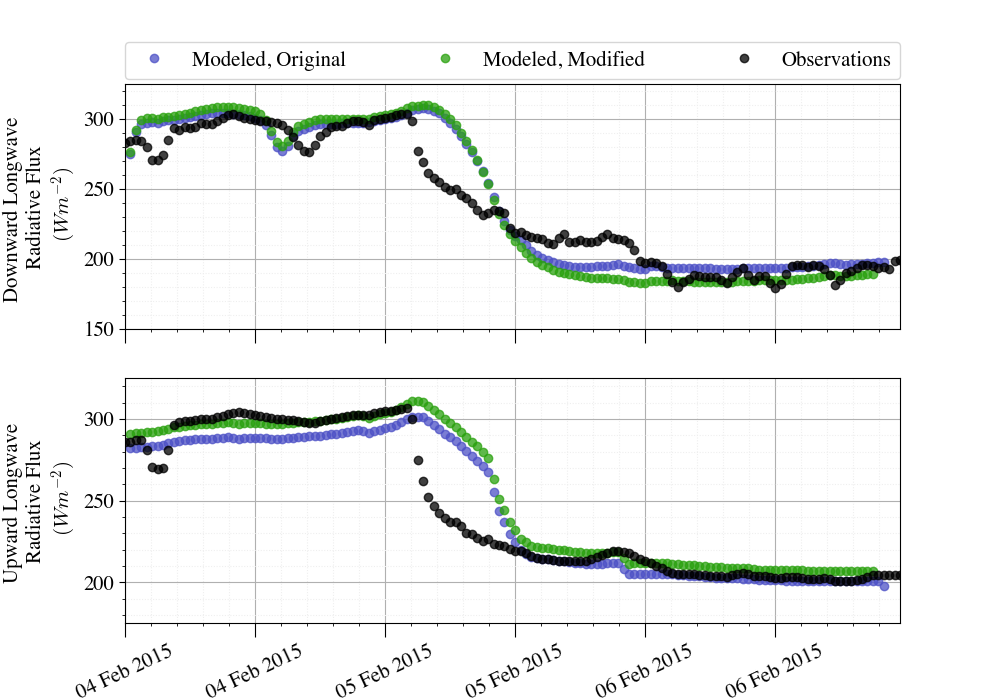
\includegraphics[width=1\linewidth]{figures/chapter6/case1_lw_sw.png}
    \caption[Idealized Case 1 - Longwave radiation.]{Upward longwave radiation (top) and downward longwave radiation (bottom) for the model with original LANDUSE.TBL values (blue), the model with modified LANDUSE.TBL values (green), and the observations (black) from 4 February to 6 February.}
    \label{fig:c1:radiative}
\end{figure}

The first case study period was from 4 February to the end of the day on 6 February. This was during a cloudy period in the winter and has been named the "Winter Cloudy" case. The downward and upward latent heat fluxes can be seen in Figure \ref{fig:c1:heat}. The modeled values do not capture the timing or sharp decrease in longwave radiation on 5 February. The modifications in the LANDUSE.TBL file do not significantly impact these fluxes, but it can be seen in Table \ref{tab:wrf:meanbias} that the modifications do reduce the mean bias in the downward longwave radiation but increase the bias in the upward longwave radiation. 

\begin{figure}[h]
    \centering
    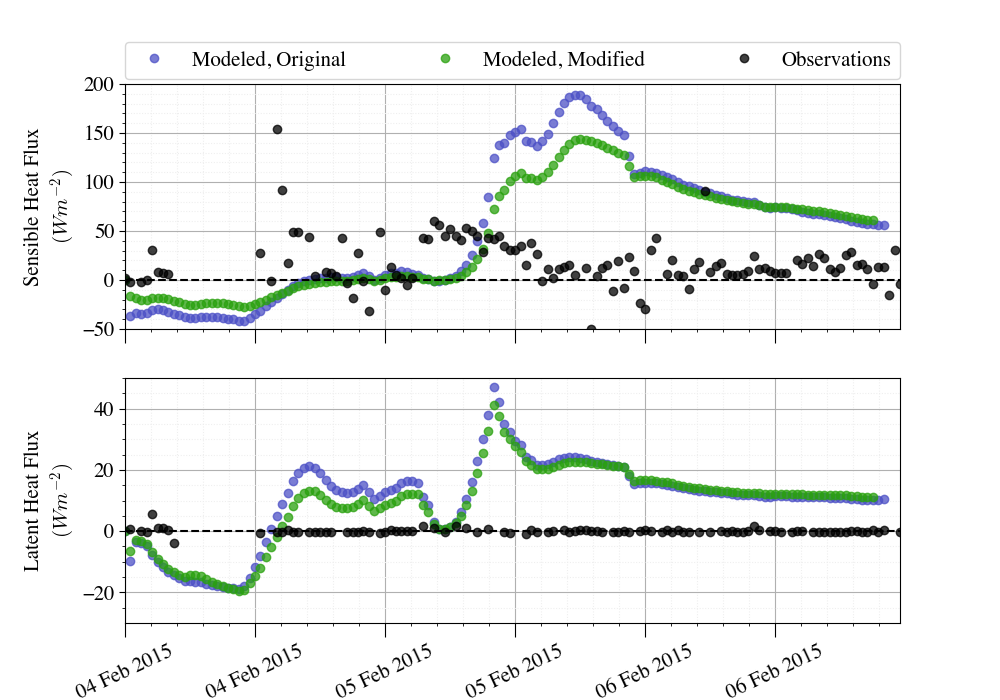
\includegraphics[width=1\linewidth]{figures/chapter6/case1_sensible_latent.png}
    \caption[Idealized Case 1 - Latent and sensible heat fluxes.]{Sensible heat flux (top) and latent heat flux (bottom) for the model with original LANDUSE.TBL values (blue), the model with modified LANDUSE.TBL values (green), and the observations (black) from 4 February to 6 February.}
    \label{fig:c1:heat}
\end{figure}

The modification in the land use table also improved latent and sensible heat flux biases. Table \ref{tab:meanbias} shows the sensible heat flux bias was reduced by almost 10 $Wm^{-2}$ in the simulations with the modified values. Latent heat flux was also improved. Figure \ref{fig:c1:heat} shows the time series of the fluxes. The modifications to the land use table do reduce the values, but they do not bring them any closer to capturing any observed patterns in the fluxes during this case.

\begin{figure}[p]
    \centering
    \vspace{-10em}
    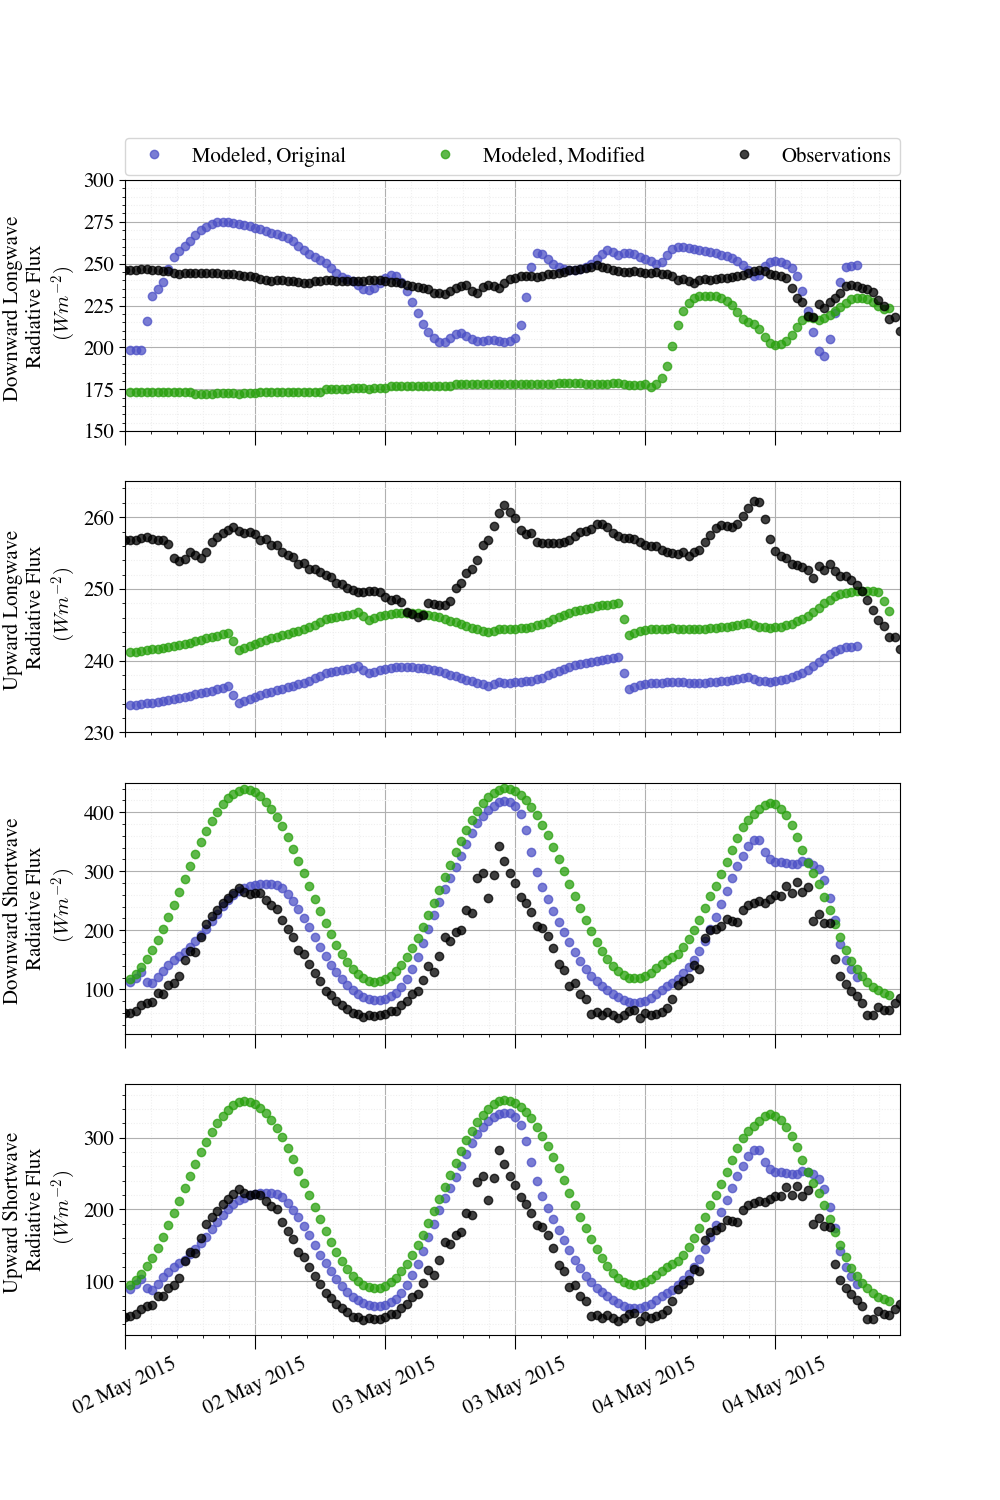
\includegraphics[width=1\linewidth]{figures/chapter6/case2_lw_sw.png}
    \caption[Idealized Case 2 - Longwave radiation.]{Upward longwave radiation (top), downward longwave radiation (second from top), upward shortwave radiation (second from bottom), and downward shortwave radiation (bottom) for the model with original LANDUSE.TBL values (blue), the model with modified LANDUSE.TBL values (green), and the observations (black) from 2 May to 4 May.}      
    \label{fig:c2:radiative}
\end{figure}

The second case study period was a cloudy period in the spring. Radiative fluxes for this period can be seen in Figure \ref{fig:c2:radiative}. At this time, the sun was rising over the N-ICE ship, so there is a shortwave component to the flux. The modified values did not do well for this case and changing the LANDUSE.TBL values removed many of the clouds during this period. While the cloud mask is not shown here, this is clear in both the longwave and shortwave radiation. The shortwave radiation (bottom panels, Figure \ref{fig:c2:radiative}) shows less radiation in the unmodified modeled results than in the modified. In fact, the unmodified results match the measurements fairly well in the shortwave. The lack of clouds in the modified simulation can also be seen in the longwave downward flux (Figure \ref{fig:c2:radiative}). These fluxes for the modified simulation are consistently much lower than those from the original runs and have little variation until the last day when the model finally begins to produce cloud cover. 

\begin{figure}[h]
    \centering
    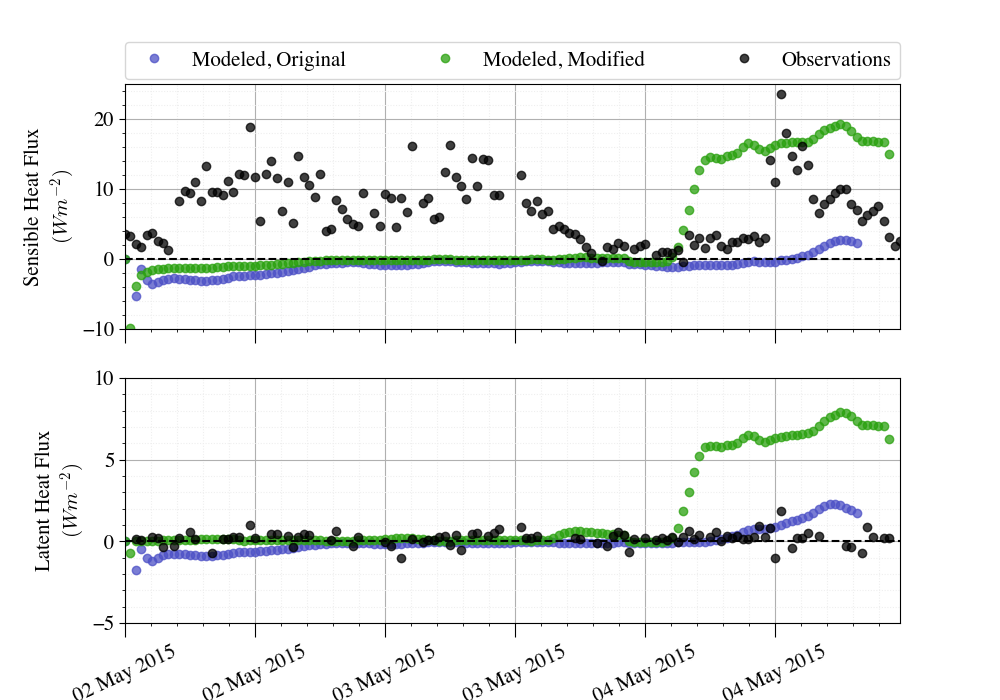
\includegraphics[width=1\linewidth]{figures/chapter6/case2_sensible_latent.png}
    \caption[Idealized Case 2 - Latent and sensible heat fluxes.]{Sensible heat flux (top) and latent heat flux (bottom) for the model with original LANDUSE.TBL values (blue), the model with modified LANDUSE.TBL values (green), and the observations (black) from 2 May to 4 May.}
    \label{fig:c2:heat}
\end{figure}

The modified LANDUSE.TBL produced higher sensible and latent heat flux values near the end of the study period (Figure \ref{fig:c2:heat}). Some increased sensible heat flux values are observed near the end of this case, and at this point, as the modified model is producing clouds and warming the air above the surface, making this the only variable and time period during this case that the modified simulation outperformed the original. Overall, mean biases (Table \ref{tab:meanbias} were higher for the model runs using the modified values than those using the original table values.

\begin{figure}[p]
    \centering
    \vspace{-10em}
    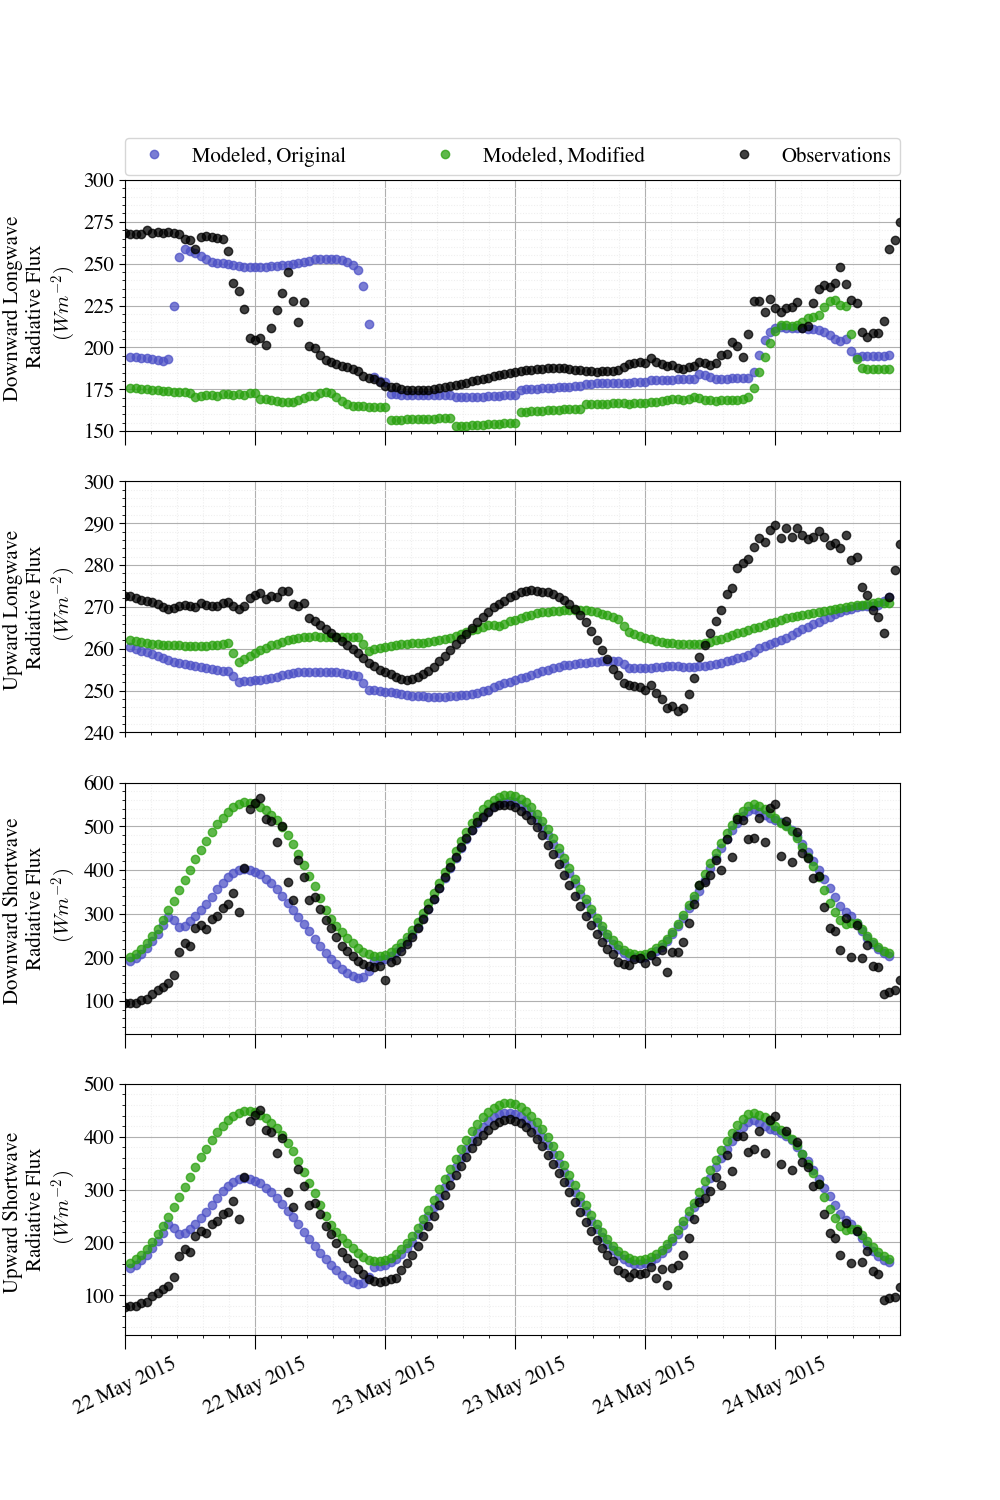
\includegraphics[width=1\linewidth]{figures/chapter6/case3_lw_sw.png}
    \caption[Idealized Case 3 - Longwave radiation.]{Upward longwave radiation (top), downward longwave radiation (second from top), upward shortwave radiation (second from bottom), and downward shortwave radiation (bottom) for the model with original LANDUSE.TBL values (blue), the model with modified LANDUSE.TBL values (green), and the observations (black) from 22 May to 24 May.}    
    \label{fig:c3:radiative}
\end{figure}

The last case study period is from 22 May to 24 May, when the N-ICE field site experienced 24 hours of cloudless skies. This 24-hour period was captured well by both the modified and unmodified simulations in the shortwave (Figure \ref{fig:c3:radiative}, bottom panels) but the day prior had some disagreement. Again, the modified simulation produced fewer clouds than those produced by the original simulations. This time, however, it matches the observations better, as the original simulation did not produce clear-sky conditions early enough in the case. The same issues can be seen with longwave radiation. Upward longwave radiation (Figure \ref{fig:c3:heat}, top) is overestimated by the original simulation for the first 24 hours of the case as the model produces clouds for too long into the evening on 22 May. The unmodified, however, does not produce enough downward longwave radiation, as this simulation did not produce enough clouds early enough. The original simulations produced lower biases for both components of shortwave radiation and the downward component up the upward radiation. Upward longwave radiation, however, had a lower bias in the modified simulation results, as the surface warmed more. 

\begin{figure}[h]
    \centering
    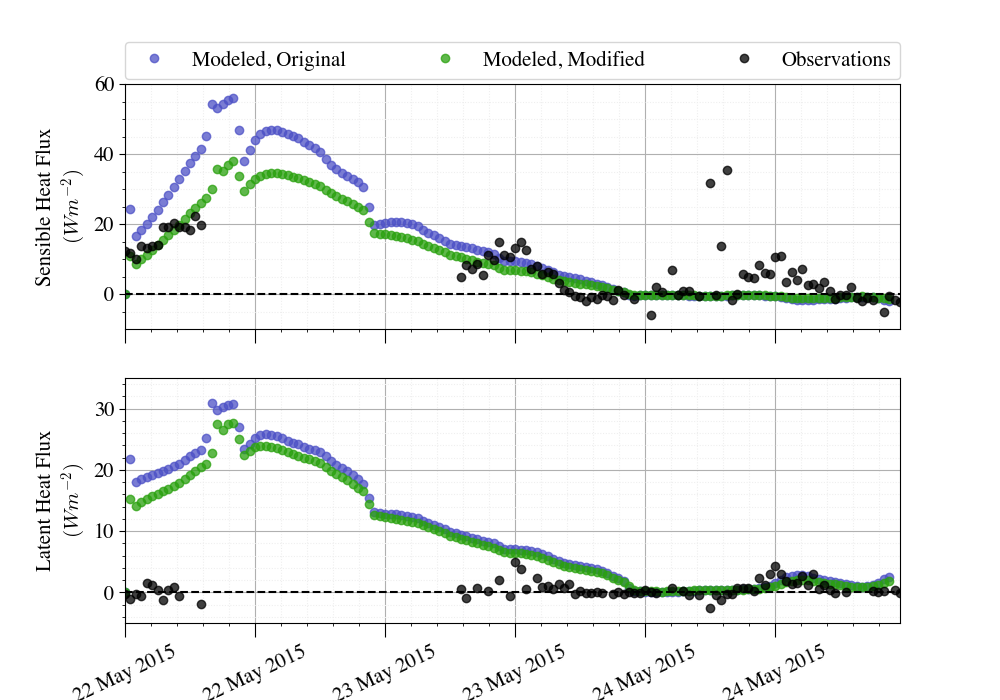
\includegraphics[width=1\linewidth]{figures/chapter6/case3_sensible_latent.png}
    \caption[Idealized Case 3 - Latent and sensible heat fluxes.]{Sensible heat flux (top) and latent heat flux (bottom) for the model with original LANDUSE.TBL values (blue), the model with modified LANDUSE.TBL values (green), and the observations (black) from 22 May to 24 May.}
    \label{fig:c3:heat}
\end{figure}

Latent and sensible heat flux values (Figure \ref{fig:c3:heat} were similar between the two model runs past the first 24 hours. They did differ during the first day when the models had disagreements about the cloud cover. The model originally overestimated these fluxes during this time period, so even a small decrease in these values could be an improvement. Table \ref{tab:meanbias} shows that the latent heat flux bias decreased by almost 1 $Wm^{2}$ with the modifications, but the sensible heat flux bias increased. 

\subsection{Flux Equations}

Throughout the entire field expedition, the WRF offline calculation did a surprisingly good job of replicating the sensible heat flux observations. Figure \ref{fig:flux:sensible} shows the observations in black and the WRF offline calculation in magenta. It is often hard to see the modeled values in the time series because they are so close to the observations that many of the points overlap each other, and they create a well-defined 1:1 line on the scatterplot. This indicates that errors in estimating the sensible heat flux are likely due to the errors in values being calculated schemes outside of the SL scheme and LSM. The WRF equation depends heavily on the friction velocity value, which is shown in Figure \ref{fig:flux:ustar}. The observed friction velocity has been calculated by the EddyPro software, and the WRF was calculated using the Polar WRF offline code using equations \ref{eq:wrf:ustar}. While WRF produces slightly smaller values of friction velocity, it is still fairly accurate throughout the entire observation period. 

\begin{table}[h]
\centering
\footnotesize
\doublespacing
{
\begin{tabular}{| c | c | c | c | c | c | c |}
\hline
\rowcolor[HTML]{F3F3F3} \textbf{Name} & \textbf{Units} & \textbf{Value} & \textbf{Source} & \textbf{Used by} \\ 
\hline
Skin temperature (surface, 2$m$, 4$m$, 10$m$) & $K$ & Variable & Measurements & \\
Pressure (sea level) & $Pa$ & Variable & Measurements & \\
Water vapor mixing ratio (2$m$, 4$m$, 10$m$) & $kg~kg^{-1}$ & & Measurements & \\
Wind speed and direction (2$m$, 4$m$, 10$m$) & $ms^{-1}$ & & Measurements & \\
Surface available moisture & & 0.5 & namelist & \\
Roughness length & $m$ & 0.15 & namelist & \\
Horizontal grid size & $m$ & 1000 & namelist & \\
Boundary layer height & $m$ & 10 & namelist & \\
\hline
\end{tabular}}
\caption{Values used by the WRF offline code.}
\label{tab:wrf:wrfsettings_offline}
\end{table}

\begin{figure}[h]
    \centering
    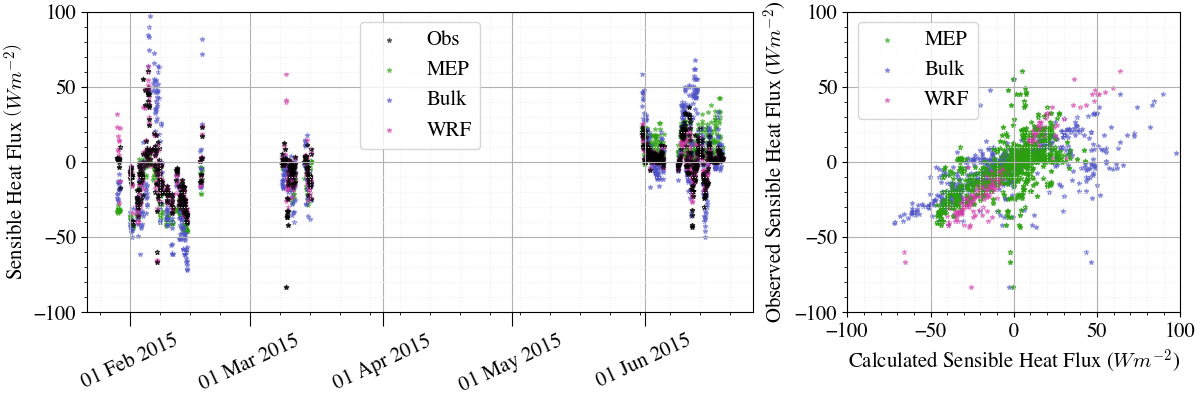
\includegraphics[width=1\linewidth]{figures/chapter6/sensible_wrf.png}
    \caption[Sensible heat flux observed at N-ICE and calculated from Polar WRF offline translated code.]{Sensible heat flux observed at N-ICE (black) and calculated from Polar WRF offline translated code (magenta), with the MEP equation (green) and with the bulk equation (blue). Scatterplot (right) shows relationships between observed and calculated values shown in the time series (left).}
    \label{fig:flux:sensible}
\end{figure}

\begin{figure}[h]
    \centering
    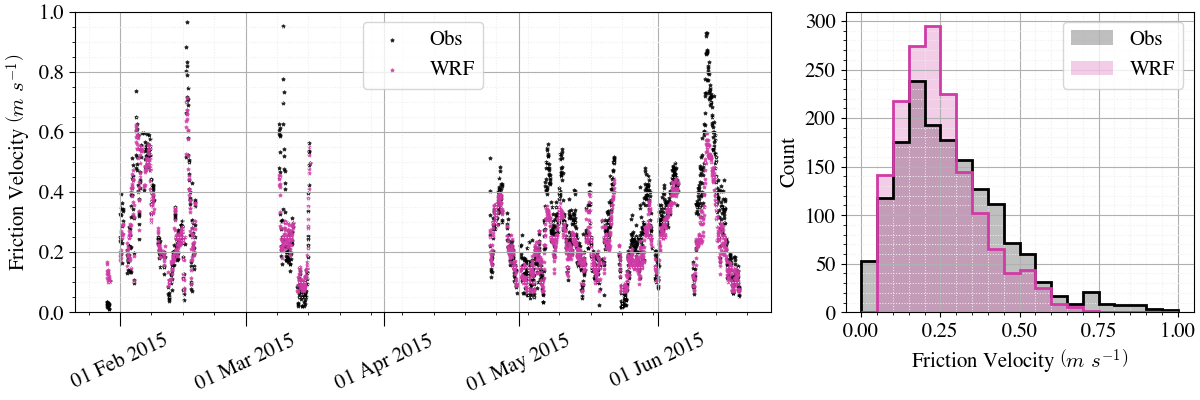
\includegraphics[width=1\linewidth]{figures/chapter6/ustar_wrf.png}
    \caption[Friction velocity observed at N-ICE and calculated from Polar WRF offline translated code.]{Friction velocity observed at N-ICE (black) and calculated from Polar WRF offline translated code (magenta).}
    \label{fig:flux:ustar}
\end{figure}

The results of the latent heat flux calculations (Figure \ref{fig:flux:latent}) do not match the observations anywhere near as well as the sensible heat flux calculations. The latent heat flux values at N-ICE were very small, and because of this, the y-axis on the scatter plot in Figure \ref{fig:flux:latent} has been reduced to -5 to 5 $Wm^{-2}$. All ways of calculating latent heat flux result in large errors, and none are able to accurately replicate the small values observed. Particularly in the summer, all equations gave largely negative latent heat flux values, but observations remained small.

\begin{figure}[h]
    \centering
    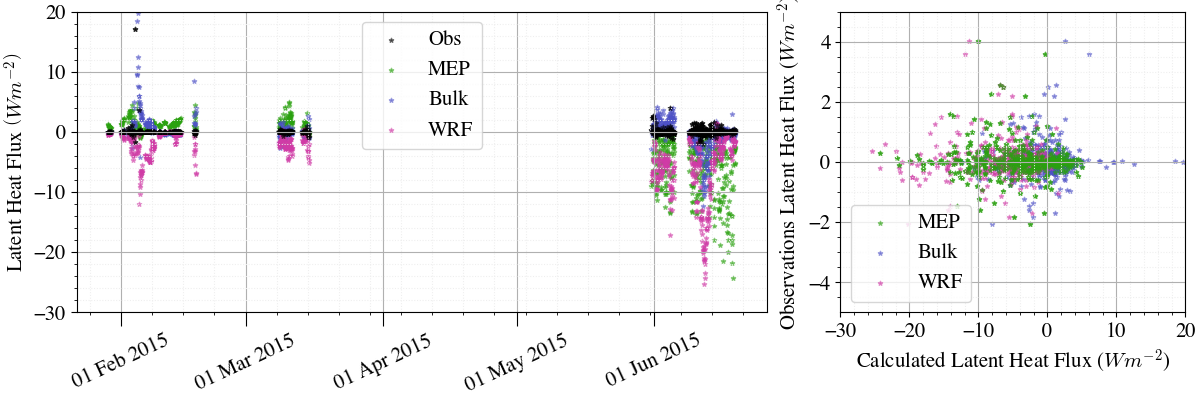
\includegraphics[width=1\linewidth]{figures/chapter6/latent_wrf.png}
    \caption[Latent heat flux observed at N-ICE and calculated from Polar WRF offline translated code.]{Latent heat flux observed at N-ICE (black) and calculated from Polar WRF offline translated code (magenta), with the MEP equation (green) and with the bulk equation (blue).  Scatterplot (right) shows relationships between observed and calculated values shown in the time series (left). Note that the y-axis (observations) in the scatterplot is scaled from -5 to 5 $Wm^{-2}$ to capture the low values observed at N-ICE.}
    \label{fig:flux:latent}
\end{figure}


\section{Final Recommendations}

\subsection{LANDUSE.TBL Changes}

More testing needs to be done to determine if these values are best under specific circumstances but using the results described above, I would recommend the following modifications be made to the LANDUSE.TBL file when working over first-year sea ice. However, I would like to also stress to the user to be mindful of the cloudiness and to be aware that these values may produce less cloud cover than using the original USGS values found in the LANDUSE.TBL.

\begin{enumerate}
  \item Increase albedo in both the winter and summer (column 3, Table \ref{tab:wrf:recommendations})
   \item Decrease surface roughness from 0.1 to 0.001 (column 5, Table \ref{tab:wrf:recommendations})
  \item Decreased surface heat capacity and use a different value for winter and summer (column 6, Table \ref{tab:wrf:recommendations})
\end{enumerate}

\subsection{Flux Equation Changes}

Latent and sensible heat flux values in WRF are calculated within the surface modules using meteorology from the BL scheme and radiation from the radiation scheme. In this study, we removed all physics schemes outside of the surface layer and created an offline, single-location model to calculate sensible and latent heat fluxes. When observed radiation, wind, temperature, and moisture values were fed into the offline model, the calculated sensible heat flux values were very accurate compared to the measurements. The latent heat flux values, however, were not, and often had significantly larger negative values than what was observed. The latent heat flux at N-ICE could not be accurately replicated by the offline WRF calculation or any of the external ways of calculating it. Chapter 3 shows that all WRF simulations struggled to replicate the latent heat flux. Chapter 4 describes several ways to calculate the latent heat flux, and none accurately represent the latent heat flux seen at N-ICE. As a result, we will focus on what we can learn from the sensible heat flux.

Chapter 3 showed that the Polar WRF model, when run as a complete model, does not accurately represent the surface conditions seen at N-ICE. The sensible heat flux had a mean bias over all model simulations of -20 $Wm^{-2}$ in the winter and 4.9 $Wm^{-2}$ in the spring. Latent heat flux had a mean bias of -0.6 $Wm^{-2}$ in the spring and 3.3 $Wm^{-2}$ in the spring. However, our offline calculations accurately simulated the sensible heat flux, indicating that something being fed into the SL scheme and LSM is a primary source of this error. Radiation is fed into the surface from the radiation scheme in WRF, but was from observations in the offline calculation. The offline calculation allows us to isolate the surface schemes and ensure any cloud-related errors are not impacting errors in the surface fluxes. The sensible heat flux errors can be attributed to errors in the longwave and shortwave radiation being read by the surface layer schemes. This radiation is likely incorrect as a result of incorrect cloud properties in the model. As described in Chapter 4, the clouds observed at N-ICE were primarily mixed phase and, as shown in Chapter 3, they were not accurately captured in any of the WRF simulations. 

